%\documentclass[uplatex,dvipdfmx,14pt]{beamer}% for 4:3
\documentclass[uplatex,dvipdfmx,14pt,aspectratio=169]{beamer}% 12pt seems common

\usepackage{bxdpx-beamer}% for dvipdfmx
\usepackage{appendixnumberbeamer}% for appendix
\usepackage{minijs}% Japanese font

%% =========================================
%% Beamer
%% =========================================
% \setbeameroption{show notes}
\setbeameroption{hide notes}

\renewcommand{\kanjifamilydefault}{\gtdefault}% Japanese to Gothic style

\usetheme[numbering=fraction,block=fill]{metropolis}% default since TeX Live 2016

\AtBeginSection[]
{
  \begin{frame}<beamer>
    \frametitle{目次}
    \tableofcontents[currentsection]
  \end{frame}
}

%% =========================================
%% Body
%% =========================================
\title{住井研究室の\\イマドキ Beamer テンプレート}
% \subtitle{}
\author{ラムダ 小太郎}
%\institute[東北大学 住井・松田研]{工学部 電気情報物理工学科\\住井・松田研究室}% 学部生
\institute[東北大学 住井・松田研]{大学院情報科学研究科 情報基礎科学専攻\\住井・松田研究室}% 院生
\date{\today}

\begin{document}

  \maketitle

  \section{foo}
  \begin{frame}{foo}
    work in progress...
    
    \note{Can you see me?}
  \end{frame}

  \section{bar}
  \begin{frame}{bar}
    \centering
    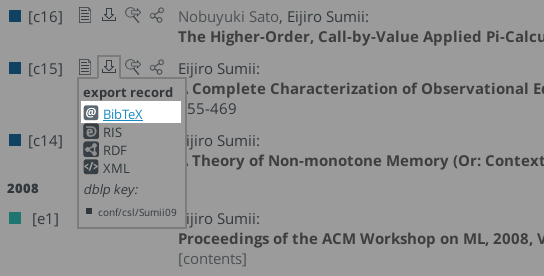
\includegraphics[scale=0.6]{../docs/dblp_bibtex_link.png}

    \note{I can see you.}
  \end{frame}

  \appendix
  \section{Appendix}
  \begin{frame}{hoge}
    Hello, world!

    \begin{block}{aaa}
      このようにして
    \end{block}
    \begin{exampleblock}{bbb}
      このようにして
    \end{exampleblock}
    \begin{alertblock}{ccc}
      このようにして
    \end{alertblock}
    
    こんにちは,世界!
  \end{frame}

\end{document}
